As artificial intelligence (AI) becomes increasingly integrated into various facets of society, it brings forth a multitude of ethical challenges that must be carefully addressed to ensure its responsible and beneficial deployment. This chapter explores some of the most critical ethical issues and risks associated with AI, drawing from both government reports and academic literature, and categorizes them into key areas of concern: transparency and explainability, data security and privacy, autonomy and accountability, bias and fairness, societal impacts, environmental concerns, and trust and control.

\section{Ethical Issues and Risks of AI}

\subsubsection{Transparency and Explainability}

One of the most pressing ethical concerns surrounding AI is the lack of transparency, often encapsulated by the term "black-box" in reference to machine learning (ML) models, particularly those based on deep neural networks. These models are complex, and their decision-making processes are often opaque, making it difficult for users, developers, and even experts to understand how specific outcomes are reached. This opacity poses significant ethical risks, as it limits the ability to scrutinize and explain the behavior of AI systems, which is crucial for ensuring accountability and building trust among users. The lack of transparency also complicates the monitoring and guidance of AI systems, increasing the risk of unintended consequences \cite{huang2022overview}.

To address these challenges, the field of explainable AI (XAI) has emerged, focusing on developing methods to make AI systems more interpretable \cite{molnar2020interpretable}. However, achieving a balance between model complexity and interpretability remains a significant hurdle. Without sufficient transparency, AI systems may be prone to errors, biases, or even manipulations that go unnoticed, leading to decisions that could have serious ethical implications.

\subsubsection{Data Security and Privacy}

AI systems are inherently data-driven, relying on vast quantities of data to learn and make decisions. This dependence on data raises profound ethical concerns regarding data security and privacy. AI systems often require access to sensitive personal information, which, if not properly protected, can be susceptible to misuse, unauthorized access, or data breaches. The collection, storage, and analysis of such data present significant privacy risks, as individuals may not always be aware of how their data is being used or who has access to it \cite{dilmaghani2019privacy}.

Moreover, the potential for malicious use of AI systems to exploit personal data is a critical ethical issue. For instance, AI technologies could be used to enhance surveillance capabilities or to develop predictive models that infringe on individuals' privacy rights. Ensuring robust data security measures and privacy protections is therefore essential in the ethical deployment of AI technologies \cite{huang2022overview}.

\subsubsection{Autonomy, Intentionality, and Accountability}

As AI systems become more autonomous, capable of making decisions without direct human intervention, the ethical challenges related to autonomy, intentionality, and accountability grow more complex \cite{sullins2011robot}. Autonomy in AI refers to the ability of a system to operate independently, making decisions and taking actions without human oversight. While this autonomy can enhance the efficiency and capabilities of AI systems, it also raises concerns about accountability. When an AI system makes a decision that leads to negative consequences, it can be difficult to determine who is responsible: the developers, the users, or the AI system itself.

This issue, often referred to as the "problem of many hands," highlights the ethical dilemma of assigning responsibility for the actions of autonomous systems \cite{timmermans2010ethics}. Moreover, the intentionality of AI systems, whether they can act in ways that are morally beneficial or harmful, further complicates the ethical landscape. Determining how much autonomy and intentionality should be granted to AI systems, and how to ensure they act in alignment with human values, are critical ethical questions that need to be addressed as AI technology continues to evolve \cite{huang2022overview}.

\subsubsection{Bias and Fairness}

Bias in AI systems is a well-recognized ethical issue that stems from both the data used to train these systems and the underlying assumptions made during their development. AI systems are only as good as the data they are trained on; if the data reflects existing societal biases, the AI systems will likely perpetuate or even exacerbate these biases. This can lead to unfair treatment of certain groups, particularly marginalized communities, in areas such as hiring, law enforcement, and access to services.

Ensuring fairness in AI is a complex task that requires ongoing efforts to identify, measure, and mitigate biases. This includes diversifying the datasets used to train AI systems, developing algorithms that can detect and correct biases, and implementing fairness audits throughout the AI lifecycle. The ethical imperative to create fair AI systems is critical, as biased AI can have significant societal implications, including reinforcing inequality and discrimination \cite{huang2022overview}.

\subsubsection{Societal Impacts: Job Displacement and Inequality}

The societal impacts of AI, particularly in terms of job displacement and increasing inequality, are among the most significant ethical concerns. As AI technologies, including robotics and automation, become more advanced, they are expected to replace many jobs, particularly those involving routine tasks. This potential for widespread job displacement raises serious ethical questions about the future of work and the societal consequences of such shifts.

Moreover, the benefits of AI are not equally distributed, potentially leading to increased inequality. Companies that can afford to implement AI technologies may gain a competitive advantage, while those that cannot may struggle to survive. This could lead to a concentration of wealth and power, exacerbating existing social and economic inequalities. The ethical challenge lies in ensuring that the development and deployment of AI contribute to societal well-being and do not disproportionately harm certain groups \cite{huang2022overview}.

\subsubsection{Environmental Concerns}

The environmental impact of AI is another critical ethical issue that warrants attention. The production and operation of AI systems, particularly those involving large-scale data processing and deep learning models, require significant amounts of energy and resources. The environmental footprint of AI includes the consumption of rare earth metals for hardware production, energy consumption for data processing, and the generation of electronic waste.

Moreover, the sustainability of AI technologies is a growing concern, as the demand for computing power continues to rise. The ethical challenge is to balance the benefits of AI with the need to minimize its environmental impact, ensuring that the development of AI technologies is aligned with broader sustainability goals \cite{huang2022overview}.

\subsubsection{Trust and Control}

Building and maintaining trust in AI systems is essential for their widespread adoption and acceptance. Trust in AI is built on several pillars, including fairness, transparency, accountability, and control. However, the increasing autonomy of AI systems, coupled with their potential to operate beyond human control, poses significant challenges to maintaining trust.

Public concerns about the controllability of AI, particularly fears of "super-intelligent" AI that could surpass human capabilities, underscore the importance of ensuring that humans retain ultimate oversight of AI technologies. Ensuring that AI systems are designed and deployed in ways that are understandable, accountable, and controllable is crucial to fostering trust and mitigating fears associated with the rise of AI \cite{huang2022overview}.

\subsection{Limitations and No Existential Risks of LLMs}

While much has been said about the potential risks posed by AI, particularly LLMs like ChatGPT, recent research suggests that fears of these models posing an existential threat to humanity may be unfounded. According to a study conducted by researchers from the University of Bath and the Technical University of Darmstadt in Germany, LLMs do not possess the capability to learn independently or acquire new skills without explicit human instruction. This inherent limitation indicates that LLMs, while highly proficient in language tasks, remain controllable, predictable, and ultimately safe for deployment.

The study highlights that LLMs excel in following instructions and generating sophisticated language based on large datasets. However, the models lack the ability to develop complex reasoning skills or master new tasks without specific guidance. This finding is significant in dispelling the notion that LLMs could evolve into uncontrollable entities capable of acting independently in ways that pose significant risks.

Dr. Harish Tayyar Madabushi, a computer scientist at the University of Bath and co-author of the study, emphasized that concerns over LLMs becoming an existential threat divert attention from more pressing issues related to AI ethics and misuse. The research demonstrated that while LLMs can perform well in familiar tasks, their limitations in reasoning and problem-solving reinforce the importance of human oversight and explicit instruction \cite{bath2024ai}.

This research underscores that while LLMs are powerful tools for language generation and task completion, they do not represent a direct threat to humanity. Instead, the focus should remain on addressing the ethical challenges associated with AI deployment, such as bias, privacy, and the potential for misuse. As Dr. Tayyar Madabushi pointed out, the real concern lies in the possibility of LLMs being used to create fake news, perpetuate fraud, or amplify harmful content—issues that require immediate attention and robust mitigation strategies \cite{lu2023emergent}.

In conclusion, while LLMs continue to advance in their linguistic capabilities, their inherent limitations provide a level of safety and control that alleviates fears of them becoming uncontrollable. Future research should prioritize addressing the genuine risks associated with AI, particularly in the context of ethical use and societal impact, rather than focusing on speculative existential threats. This approach will ensure that AI technologies can be developed and deployed responsibly, maximizing their benefits while minimizing potential harms.

\section{Global AI Regulations}

As artificial intelligence (AI) continues to advance and integrate into various aspects of society, the need for robust regulatory frameworks becomes increasingly evident. Around the world, governments and international organizations are grappling with the challenges of creating policies that balance innovation with ethical considerations, safety, and public trust. The map in Figure \ref{fig:AI_regulations_world} illustrates the number of AI-related bills passed into law by different countries from 2016 to 2023, highlighting the global momentum towards regulating AI technologies.

\begin{figure}[h!]
    \centering
    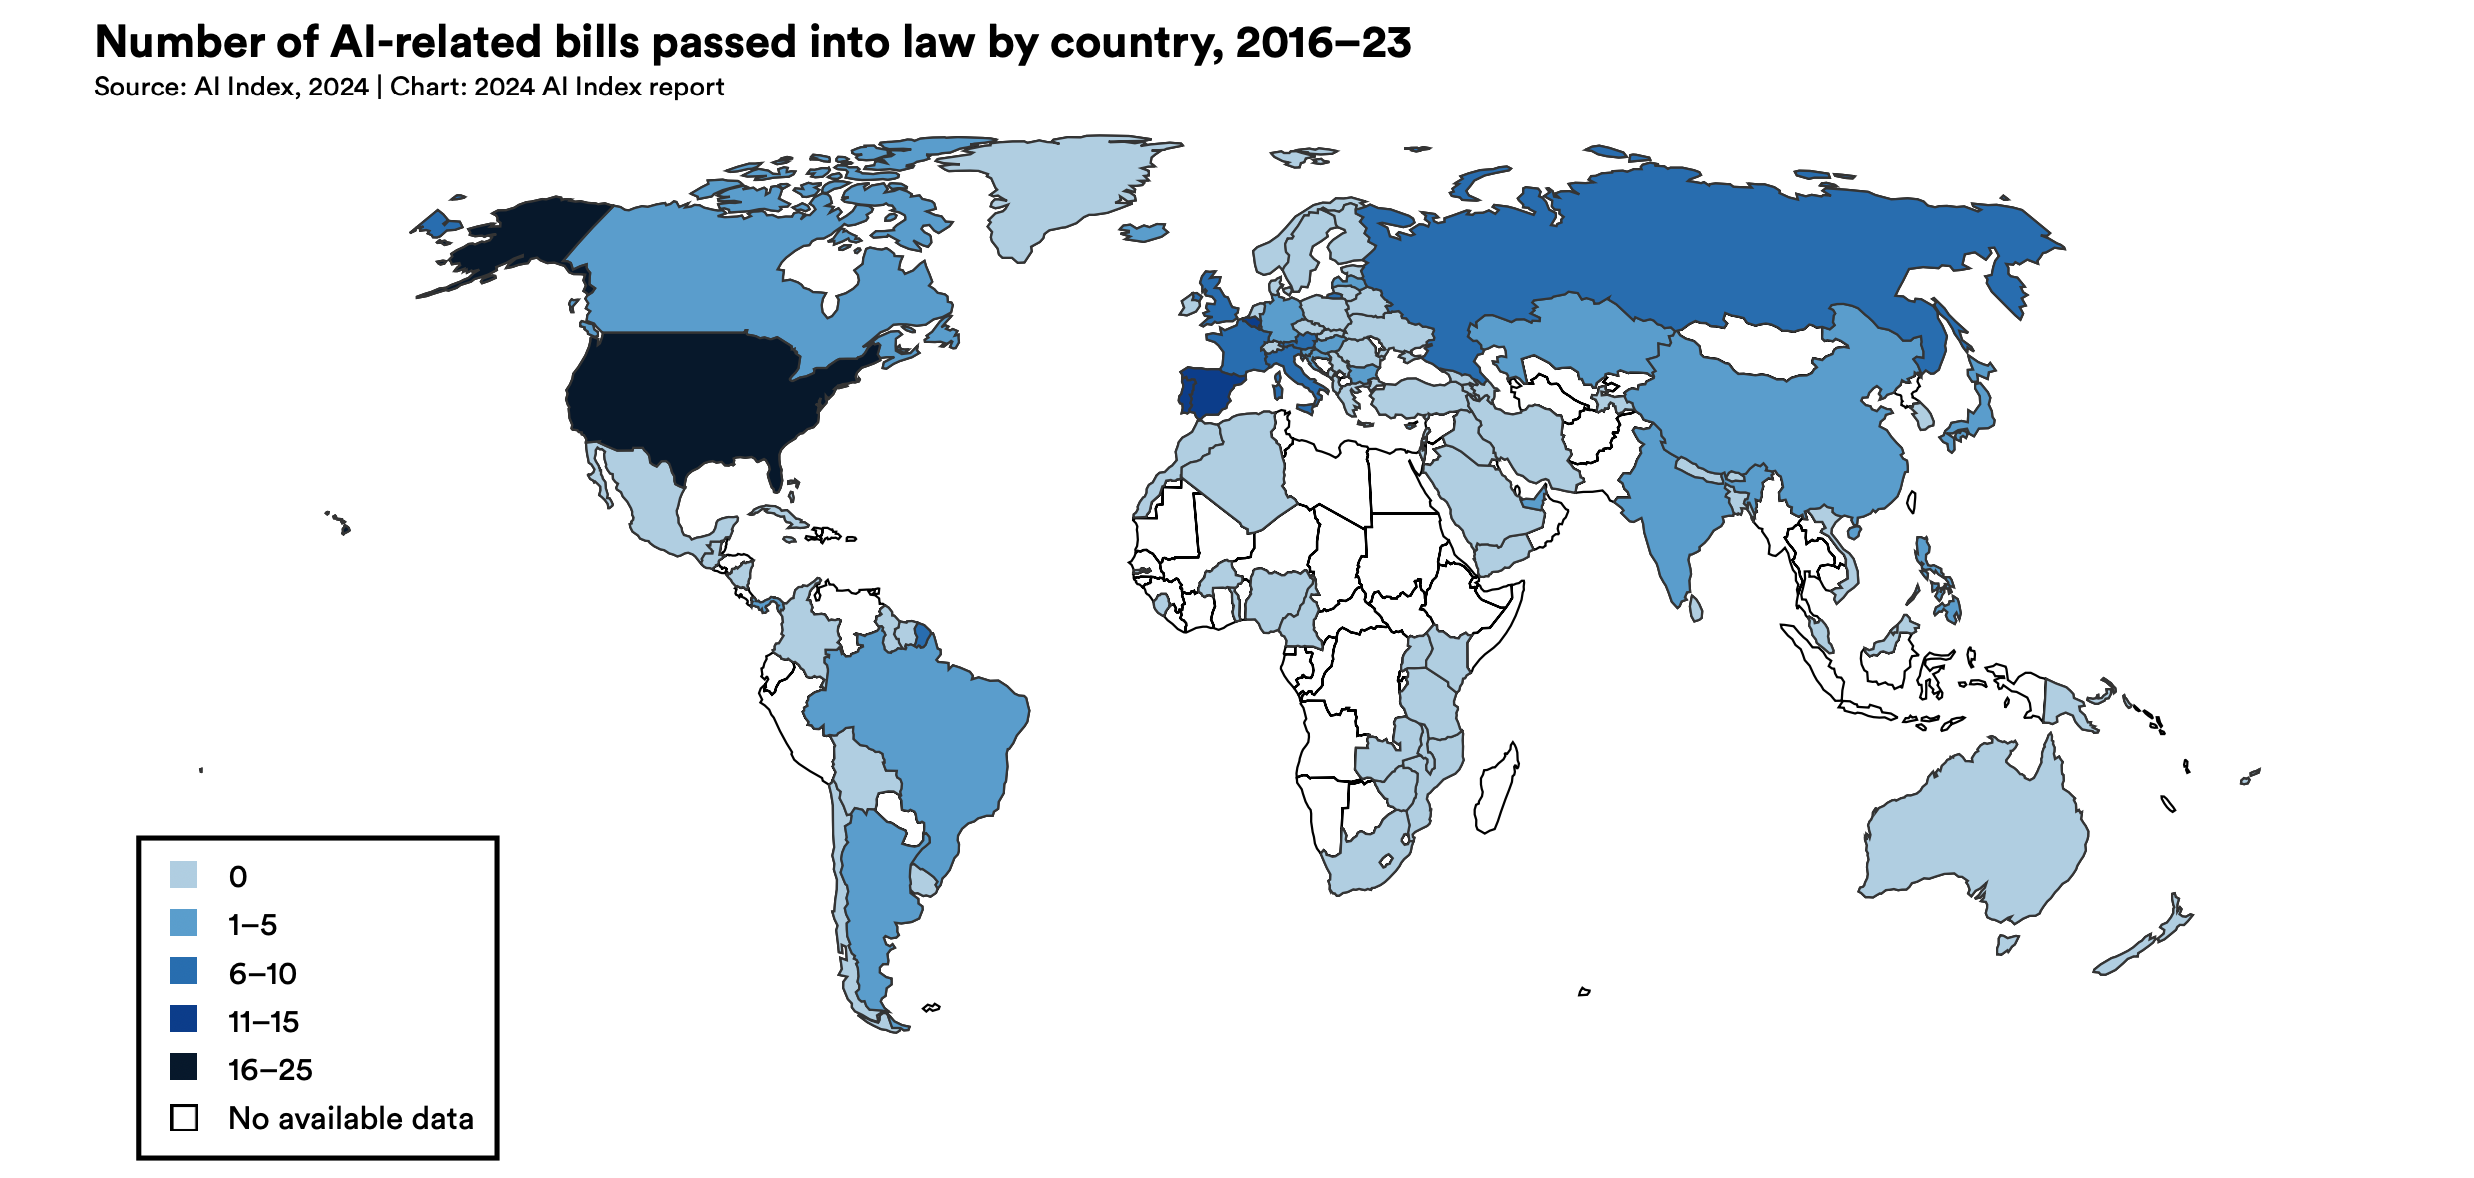
\includegraphics[width=0.9\textwidth]{images/regulation/world-AI-regulation.png}
    \caption{Number of AI-related bills passed into law by country, 2016–2023 \textit{Source:} \cite{maslej2024ai}}
    \label{fig:AI_regulations_world}
\end{figure}

As illustrated in Figure \ref{fig:AI_regulations_world}, since early 2016, numerous national, regional, and international authorities have initiated the adoption of strategies, action plans, and policy frameworks pertaining to AI governance \cite{berryhill2019hello}. Diverse nations have embraced distinct regulatory paradigms to address AI, with significant variation observed in the approaches of the world’s three largest economies. Notably, the United States is characterized by a market-driven regulatory approach, China by a state-centric strategy, and the European Union by a rights-oriented framework \cite{allen2023race}.These efforts reflect the growing recognition of the need to regulate AI to address its ethical implications, ensure privacy, and protect human rights. This section proceeds by examining the regulatory approaches of these key global actors: the European Union’s comprehensive and rights-focused framework exemplified by the AI Act, the United States’ market-driven approach with a strong emphasis on innovation and regulatory oversight, and China’s state-driven strategy that integrates AI development within its broader national objectives.

\subsection{The AI Act and Beyond: The European Union's Leadership in AI Regulation}

The European Union (EU) has positioned itself as a global leader in the regulation of digital technologies, including AI. Through its comprehensive legislative framework, the EU seeks to balance the promotion of innovation with the protection of fundamental rights and values. Among its significant regulatory achievements are the General Data Protection Regulation (GDPR) \cite{cepr_gdpr_2023}, the Digital Services Act (DSA), and the Digital Markets Act (DMA), which collectively form a robust foundation for digital governance. In 2023, the EU's Artificial Intelligence Act (AI Act) was recognized as the most far-reaching regulation of AI worldwide, underscoring the EU's commitment to shaping the global landscape of AI governance \cite{nyt_europe_ai_regulation_2023}.

While individual EU member states have developed their own national AI strategies, these are largely aligned with the broader European Strategy on AI. This strategy is supported by a High-Level Expert Group on AI, which provides guidance on ethical and trustworthy AI. In 2019, the European Commission published its \textit{Ethics Guidelines for Trustworthy Artificial Intelligence} \cite{eu_trustworthy_ai_2019}, followed by \textit{Policy and investment recommendations aimed at fostering trustworthy Artificial Intelligence} \cite{eu_ai_investment_2019}. These efforts have laid the groundwork for a cohesive approach to AI regulation across the EU.

A key milestone in the EU's AI regulatory journey was the publication of the White Paper on Artificial Intelligence in February 2020 \cite{eu_white_paper_ai_2020}. This document outlined the EU's dual approach, focusing on creating an "ecosystem of excellence" to promote innovation, and an "ecosystem of trust" to establish a robust regulatory framework. Central to this framework is the classification of AI applications based on risk. The EU's regulatory approach distinguishes between high-risk AI applications, those operating in sectors such as healthcare, transport, and energy, and applications that pose minimal or limited risk. High-risk AI systems are subject to stringent requirements, including the need for high-quality training data, robust data management practices, and human oversight. For AI applications deemed to pose minimal or limited risk, a voluntary labeling scheme is proposed, providing flexibility while encouraging compliance with best practices \cite{mhc_regulating_ai_2023}.

The legislative process for the AI Act has been dynamic, with the initial draft presented in April 2021 and the final version adopted in May 2024. The AI Act introduces a refined risk-based approach with four categories: minimal, limited, high, and unacceptable risk. High-risk AI systems, such as those used in critical infrastructure and law enforcement, are subject to stringent obligations, including rigorous risk assessments, the use of high-quality datasets, traceability requirements, and human oversight. Limited risk AI systems, such as chatbots, are required to maintain transparency, ensuring that users are aware they are interacting with a machine. Lastly, minimal-risk AI systems, such as video games or spam filters, can be freely developed and used without significant regulatory constraints. Notably, the AI Act also addresses general-purpose AI models, such as ChatGPT, which do not fit neatly into application-based regulatory frameworks \cite{reuters_eu_ai_rules_2023}. These models are regulated based on their capabilities, with transparency requirements for weaker models and stringent evaluations for those posing systemic risks.

The AI Act's emphasis on non-discrimination and fairness is particularly pertinent for the development of AI chatbots. Developers are required to mitigate biases in these models by employing diverse and inclusive training datasets and regularly reviewing and updating the AI models to ensure compliance with ethical standards.

The AI Act also includes provisions prohibiting certain AI applications, such as real-time remote biometric identification and emotion recognition, with specific exemptions for law enforcement. The gradual enforcement of the AI Act reflects the EU's cautious approach to balancing innovation with the protection of citizens' rights \cite{atlantic_council_eu_ai_rules_2023}.

Penalties for non-compliance with the AI Act are significant, with fines based on a company’s global annual turnover. The fines vary depending on the severity of the violation, with higher penalties for breaches involving banned AI applications or failure to meet the Act’s obligations. These fines aim to ensure that companies adhere to the regulations, though there is ongoing debate about whether the penalties are too strict or necessary to ensure trustworthy AI development.

However, the rapid pace of legislative initiatives under the von der Leyen Commission has raised concerns about potential risks to digital rights, particularly regarding privacy and data protection. Critics have pointed to the challenges of ensuring effective coordination between EU measures and national strategies, as well as the need for stronger governance to monitor investments and implementation \cite{wikipedia_ai_regulation}.

The AI Act, as part of the broader EU strategy, reflects the Union's ambitions for strategic autonomy and digital sovereignty. By establishing a comprehensive and forward-looking regulatory framework, the EU aims to lead the global discourse on AI governance, ensuring that AI technologies are developed and deployed in a manner that aligns with European values and fundamental rights. As the AI Act is progressively enforced, it will likely serve as a model for AI regulation in other regions, further cementing the EU's role as a global regulator in the digital age.

\subsection{AI Regulation in the United States }

The United States has approached the regulation of AI with a focus on balancing innovation with the need for oversight in a rapidly evolving technological landscape. Discussions surrounding AI regulation in the U.S. have primarily revolved around determining the appropriate federal framework, the roles of various government agencies, and the challenges of updating regulations in response to technological advancements \cite{weaver2018regulation}.

The initial steps towards AI regulation in the U.S. can be traced back to the Obama administration's 2016 report, \textit{Preparing For the Future of Artificial Intelligence}, which emphasized the importance of allowing continued AI research and development with minimal restrictions, while also recognizing the need to assess potential risks associated with AI technologies. This report set the stage for a regulatory approach that prioritizes public safety and encourages innovation \cite{obama_ai_2016}.

In subsequent years, several significant legislative and policy initiatives have shaped the U.S. approach to AI. The establishment of the National Security Commission on Artificial Intelligence in 2018 marked a critical step in addressing AI's implications for national security and defense. This commission has played a pivotal role in guiding the development and regulation of security-related AI applications \cite{nscai_2021}.

Under the Trump administration, the \textit{Executive Order on Maintaining American Leadership in Artificial Intelligence} was issued in January 2019, leading to the release of the \textit{Guidance for Regulation of Artificial Intelligence Applications} \cite{executive_order_maintaining_ai_leadership_2019, omb_memo_regulation_ai_2020}. This guidance, along with input from agencies such as the National Institute of Standards and Technology (NIST) and the Defense Innovation Board, laid out principles for federal agencies to consider when regulating AI, with a focus on ensuring safety, fairness, and transparency \cite{wikipedia_ai_regulation}.

In more recent years, the Biden administration has taken proactive steps towards AI regulation. In October 2022, President Biden introduced the AI Bill of Rights, outlining five key protections for Americans in the AI era, including safe and effective systems, protection against algorithmic discrimination, data privacy, transparency, and human oversight. This initiative underscores the administration's commitment to safeguarding civil rights and ensuring that AI technologies are developed and used responsibly \cite{ai_bill_of_rights_2022}.

The administration has also secured voluntary commitments from major tech companies to manage AI risks, focusing on security testing, information sharing, and addressing societal challenges posed by AI, such as bias and privacy concerns. Furthermore, the release of the \textit{Executive Order on Safe, Secure, and Trustworthy Artificial Intelligence} in October 2023 marked a significant advancement in the U.S. regulatory landscape. This order grants various federal agencies the authority to apply consumer protection laws to AI development and emphasizes the importance of equity, civil rights, and job quality in AI applications \cite{biden_executive_order_ai_2023}.

The regulatory landscape in the United States continues to evolve as both federal and state governments grapple with the complexities of AI governance. These efforts reflect a growing recognition of the need to balance innovation with ethical considerations, ensuring that AI technologies are developed in a manner that aligns with American values and priorities.

\subsection{AI Regulation in China}

The regulation of artificial intelligence (AI) in China is predominantly governed by the State Council of the People's Republic of China, under the "Next Generation Artificial Intelligence Development Plan", issued on July 8, 2017. This plan, endorsed by the Central Committee of the Chinese Communist Party and the State Council, outlines a strategic roadmap for AI development in China, with goals extending to 2030. The plan emphasizes the importance of AI as a key driver of economic transformation and innovation, urging the country's governing bodies to foster the advancement of AI technologies \cite{china_ai_plan_2017}.

China's regulatory approach to AI is characterized by stringent state control over both domestic companies and data, particularly regarding the storage and handling of data on Chinese users. The regulatory framework mandates that AI systems and related technologies comply with the national standards of the People's Republic of China, covering areas such as big data, cloud computing, and industrial software. This centralized approach reflects the broader strategy of ensuring that AI development aligns with the state's objectives and security concerns \cite{wu2020towards}.

In 2021, China published ethical guidelines for AI usage, stipulating that AI systems must adhere to shared human values, remain under human oversight, and avoid endangering public safety. These guidelines underscore the importance of ethical considerations in AI development, particularly in ensuring that AI technologies contribute positively to society and do not pose risks to individuals or the public \cite{cset_ethical_norms_2021}.

Further expanding its regulatory framework, China introduced the "Interim Measures for the Management of Generative AI Services" in 2023 \cite{fortune_china_ai_2023}. These measures reflect China's proactive stance in addressing the rapidly evolving field of generative AI, setting forth regulations to manage the deployment and operation of these technologies within the country. The measures are part of China's broader effort to maintain control over AI development and ensure that such technologies are developed and used in ways that align with national interests and ethical standards.
